\begin{center}
	\bigskip \bigskip \bigskip \bigskip
	{\huge \bf Appendix} \\
	\bigskip \bigskip
\end{center}
\addcontentsline{toc}{section}{Appendix}

\section{Appendix A}

\subsection{Illustrations}
\label{appendix:illustrations}

Illustrations as found in~\cite{kraemer-oppidum-maching}.

\begin{figure}[ht]
	\centering
	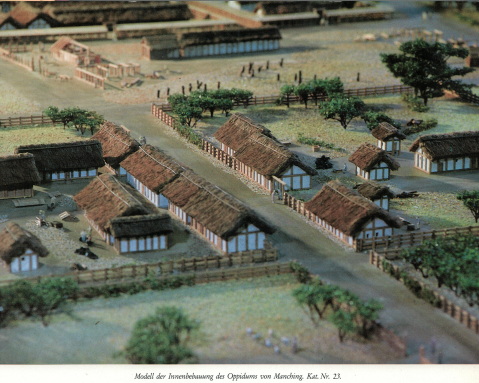
\includegraphics[width=\linewidth]{pictures/scan_manching_2.png}
	\caption{Model of the inner buildings of the  Oppodium of Manching.}
\end{figure}

\begin{figure}[ht]
	\centering
	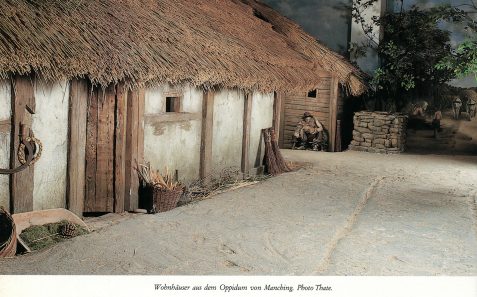
\includegraphics[width=\linewidth]{pictures/scan_manching_1.png}
	\caption{A illustration of a living house.}
\end{figure}

\begin{figure}[ht]
	\centering
	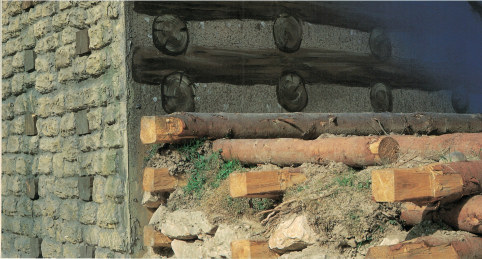
\includegraphics[width=\linewidth]{pictures/scan_manching_4.png}
	\caption{Construction of a wall.}
\end{figure}


\begin{figure}[ht]
	\centering
	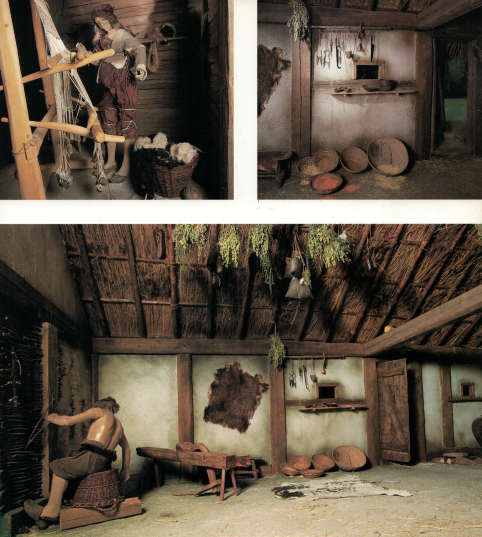
\includegraphics[width=\linewidth]{pictures/scan_manching_3.png}
	\caption{Inner view of a living house.}
\end{figure}

\clearpage
\pagebreak
Illustrations from Rieckhoff and Biel's \textit{'Die Kelten in Deutschland`}~\cite{rieckhoff-walls1}\cite{rieckhoff-walls2}\cite{rieckhoff-tower}.

\begin{figure}[ht]
	\centering
	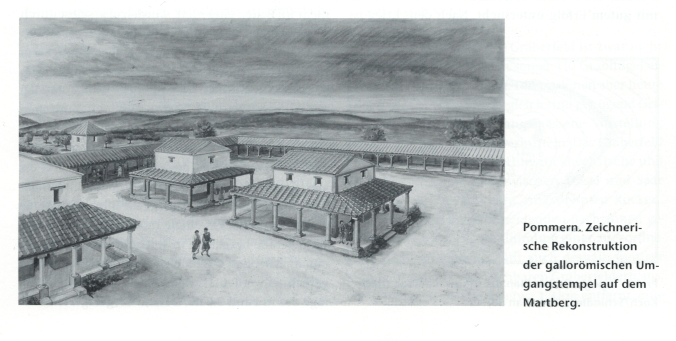
\includegraphics[width=\linewidth]{pictures/scan_rieckhoff_tower.png}
	\caption{We modeled our tower after the tower on the left of the background.}
\end{figure}

\begin{figure}[ht]
	\centering
	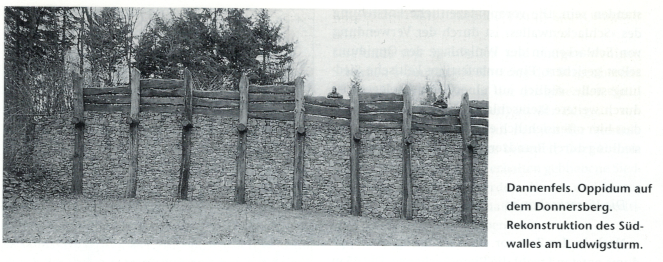
\includegraphics[width=\linewidth]{pictures/scan_rieckhoff_wall1.png}
	\caption{Reconstruction of a Oppidum wall.}
\end{figure}

\begin{figure}[ht]
	\centering
	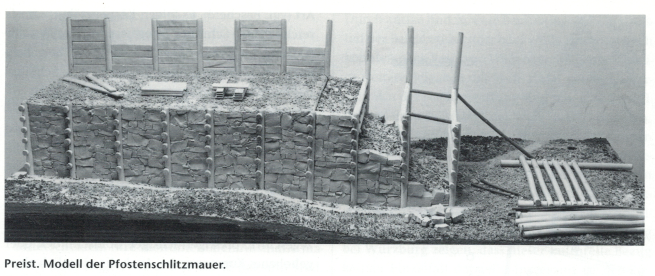
\includegraphics[width=\linewidth]{pictures/scan_rieckhoff_wall2.png}
	\caption{Another reconstruction of an Oppidum wall.}
\end{figure}

\begin{figure}[ht]
	\centering
	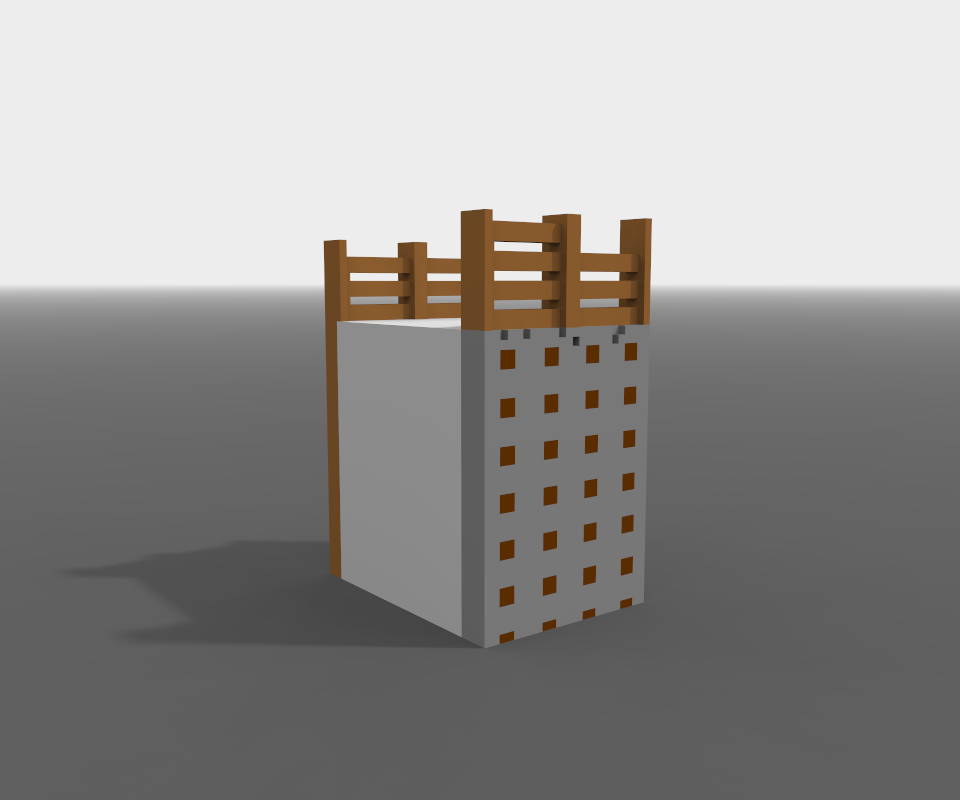
\includegraphics[width=\linewidth]{pictures/stone_wall.png}
	\caption{Our stone wall model.}
\end{figure}
